\subsection[Baum-Welch algorithm]{Learning from Observations:
  Baum-Welch algorithm}
\label{sec:bw}

\begin{frame}[t]
	\frametitle{Learning from observations - Reminder}
	\begin{block}{Model Estimation (Training) Problem}
    	Given some observed sequences, how do we adjust the \alert{parameters} of an HMM model that best tries 	
    	to explain the observations?
  	\end{block}
  	\pause
  	
  	\begin{block}{}
  		Adjust the model parameters $\lambda = (A, B, \Pi)$ to obtain $\max_{\lambda} P(O \vert \lambda)$
  	\end{block}
  	\pause
  	
  	\begin{block}{}
  		The observation sequence used to adjust the model parameters is called a \alert{training} sequence.\\
  		Training problem is crucial - allows to create best models for real phenomena.
  	\end{block}
\end{frame}


\begin{frame}[t]
	\frametitle{Learning from observations - Aspects of the approach}
	\pause
		
	\begin{block}{\alert{Problem}}
    	There is no known way to analytically solve for the model which maximizes the probability of the
    	observation sequence.
  	\end{block}
  	\pause
  	
  	\begin{block}{Solution}
  		We can choose $\lambda = (A, B, \Pi)$ such that $\max_{\lambda} P(O \vert \lambda)$ is 
  		\alert{locally maximized} using an \alert{iterative procedure} such as \emph{Baum-Welch}.\\
  		The method is an instance of the \emph{EM algoritm} \parencite{dempster1977maximum} for HMMs.
  	\end{block}
  	
\end{frame}

\begin{frame}[t]
	\frametitle{Baum-Welch algorithm (I)}
	\pause
	We first define some auxiliary values:
	
	\begin{block}{}    
    	$\xi_{t,i,j} = \xi_t(i,j) = P(q_t=s_i,q_{t+1}=s_j \vert O, \lambda)$\\
    	The probability of being in state $s_i$ at time $t$ and in state $s_j$ at time $t+1$, given
    	the model and the observation sequence.
	\end{block}
	\pause
	
	\begin{block}{}    
    	$ \gamma_{t,i} = \gamma_t(i) = P(q_t = s_i \vert O, \lambda)$\\
    	The probability of being in state $s_i$ at time $t$, given the model and the observation sequence.
	\end{block}
	\vspace*{1em}
	\pause
	
	From the definitions it follows that:\\
	$ \gamma_t(i) = \displaystyle\sum_{j=1}^{N}\xi_t(i,j)$
  	
\end{frame}

\begin{frame}[t]
	\frametitle{Baum-Welch algorithm (II)}
	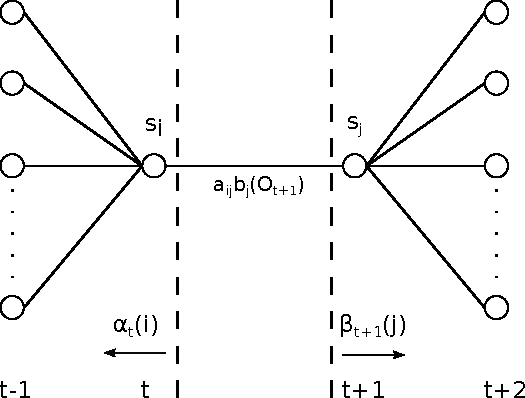
\includegraphics[height=0.35\textheight]{images/baum-welch-alg.pdf}
  	
\end{frame}